%                      Code_Saturne version 1.3
%                      ------------------------
%
%     This file is part of the Code_Saturne Kernel, element of the
%     Code_Saturne CFD tool.
% 
%     Copyright (C) 1998-2007 EDF S.A., France
%
%     contact: saturne-support@edf.fr
% 
%     The Code_Saturne Kernel is free software; you can redistribute it
%     and/or modify it under the terms of the GNU General Public License
%     as published by the Free Software Foundation; either version 2 of
%     the License, or (at your option) any later version.
% 
%     The Code_Saturne Kernel is distributed in the hope that it will be
%     useful, but WITHOUT ANY WARRANTY; without even the implied warranty
%     of MERCHANTABILITY or FITNESS FOR A PARTICULAR PURPOSE.  See the
%     GNU General Public License for more details.
% 
%     You should have received a copy of the GNU General Public License
%     along with the Code_Saturne Kernel; if not, write to the
%     Free Software Foundation, Inc.,
%     51 Franklin St, Fifth Floor,
%     Boston, MA  02110-1301  USA
%
%-----------------------------------------------------------------------
%

%%%%%%%%%%%%%%%%%%%%%%%%%%%%%%%%%%
%%%%%%%%%%%%%%%%%%%%%%%%%%%%%%%%%%
\section{Mise en \oe uvre}
%%%%%%%%%%%%%%%%%%%%%%%%%%%%%%%%%%
%%%%%%%%%%%%%%%%%%%%%%%%%%%%%%%%%%

%\etape{Mode de prescription des conditions aux limites\vspace{0,3cm}}
%%%%%%%%%%%%%%%%%%%%%%%%%%%%%%%%%%%%%%%%%%%%%%%%%%%%%%%%%%%%%%%%%%%%
On traite ici les variables \var{IVAR} sur les faces \var{IFAC} 
telles que \var{ICODCL(IFAC,IVAR)}=5. 

La vitesse de d\'efilement (\'eventuellement nulle) de la paroi est tout d'abord
projet\'ee dans le plan tangent \`a la paroi. Ses trois composantes dans le
rep\`ere de calcul sont stock\'ees dans les
tableaux\\  \var{RCODCL(IFAC,IUIPH,1),RCODCL(IFAC,IVIPH,1)RCODCL(IFAC,IWIPH,1)}. 

On d\'etermine ensuite le
rep\`ere local $\hat{\mathcal R}$. Pour chaque face, il est disponible dans les
vecteurs $\vect{\tau}$ \var{(TX, TY, TZ)}, $\vect{\tilde{n}}$ \var{(-RNX, -RNY,
-RNZ)}, et $\vect{b}$ \var{(T2X, -T2Y,-T2Z)}. Il faut noter que le troisi\`eme
vecteur n'est n\'ecessaire (et n'est donc calcul\'e) que lorsque le mod\`ele de
turbulence $R_{ij}-\varepsilon$ est utilis\'e (pour la projection du tenseur
d'ordre deux). Par ailleurs, si la norme de la vitesse
tangentielle est inf\'erieure \`a la valeur arbitraire \var{EPZERO}
($10^{-12}$), l'indicateur \var{TXN0} est positionn\'e \`a 0 (il vaut 1 sinon)
et le vecteur $\vect{\tau}$ est pris 
\begin{itemize}
\item [-] arbitraire, dans le plan perpendiculaire \`a $\vect{\tilde{n}}$ en
$R_{ij}-\varepsilon$  (on utilise les composantes de $\vect{\tilde{n}}$ pour
construire  $\vect{\tau}$~; si  $\vect{\tilde{n}}$ est identiquement nul, le
code s'arr\^ete)~;
\item [-] identiquement nul sinon.
\end{itemize}

Une fois le rep\`ere local d\'etermin\'e, le sous-programme \fort{clca66} est
appel\'e avec\footnote{\var{CLSYME} = 0 permet de sp\'ecifier qu'on
traite les conditions de paroi et non des conditions de sym\'etrie. On pourra se
reporter \`a \var{CLSYVT} pour les d\'etails de \fort{clca66}.} \var{CLSYME} =0
si le mod\`ele $R_{ij}-\varepsilon$ est activ\'e, afin de calculer la
matrice \var{ALPHA} qui permettra, \`a partir des valeurs du tenseur de Reynolds
au points $I'$, de calculer les valeurs \`a imposer aux faces de bord. 

On calcule ensuite les vitesses de frottement qui sont stock\'ees dans
\var{UET} ($=u^*$) et dans \var{UK} ($=u_k$). Le sous-programme \fort{causta}
 permet de calculer la vitesse de 
frottement pour le mod\`ele \`a une \'echelle
de vitesse (\var{IDEUCH}=0). Pour le mod\`ele \`a deux \'echelles
(\var{IDEUCH}=1), le calcul (plus simple) de \var{UET} et de \var{UK} est fait directement
dans \fort{clptur}. Le sous-programme utilisateur \fort{usruet} permet alors de
donner la main \`a l'utilisateur qui souhaiterait  modifier les \'echelles de
vitesses (prise en compte d'une paroi rugueuse, ou de variantes de
la loi logarithmique par exemple). 

Dans le cas ou le mod\`ele \`a une \'echelle de vitesse est actif, on impose
\var{UK=UET} afin de conserver la coh\'erence du codage dans la suite du
sous-programme. N\'eanmoins, dans le cas o\`u on se trouve dans la sous-couche visqueuse, on force \var{UK=0} ce qui
permettra d'obtenir une valeur nulle pour $k$ et un flux nul pour $\varepsilon$
(la valeur \var{UET} n'est pas utilis\'ee, car la condition sur la vitesse
devient une condition d'adh\'erence et les tensions de Reynolds sont annul\'ees).
Si l'on se trouve dans la sous-couche visqueuse, on recalcule \var{UET} 
(et \var{YPLUS} si l'on est \`a une \'echelle de vitesse) car l'\'evaluation 
pr\'ec\'edente a \'et\'e faite avec l'hypoth\`ese que l'on \'etait en zone 
logarithmique.

Les conditions aux limites pour la vitesse sont ensuite compl\'et\'ees.
\begin{itemize}

\item [-] En $k-\varepsilon$, on affecte, pour les trois composantes de vitesse
respectivement, \`a $$\var{COEFA(IFAC,ICLUF)}, \var{COEFA(IFAC,ICLVF)} \,\text{ et
}\,\var{COEFA(IFAC,ICLWF)}$$ les coefficients $A_{flux}$  
issus de l'analyse relative \`a la contrainte tangentielle.\\
 De m\^eme, les coefficients $B_{flux}$ sont affect\'es \`a
$$\var{COEFB(IFAC,ICLUF)}, \var{COEFB(IFAC,ICLVF)} \,\text{ et
}\,\var{COEFB(IFAC,ICLWF)}.$$ Les conditions aux limites
issues de l'analyse portant directement sur le gradient de vitesse $A_{grad}$ et
$B_{grad}$ sont affect\'ees \`a  $$\var{COEFA(IFAC,ICLU)},
\var{COEFA(IFAC,ICLV)}, \var{COEFA(IFAC,ICLW)}$$ et
$$\var{COEFB(IFAC,ICLU)}, \var{COEFB(IFAC,ICLV)}, \var{COEFB(IFAC,ICLW)}.$$ 

\item [-] Lorsque la vitesse tangentielle en $I'$ est inf\'erieure \`a
\var{EPZERO}, l'indicateur \var{TXN0} est annul\'e (sinon,  \var{TXN0} vaut 1). 
De m\^eme, quand la valeur de
$y^+$ est inf\'erieure ou \'egale \`a $10,88$, l'indicateur
\var{UNTURB} est positionn\'e \`a 0 (sinon, il vaut 1). Ces deux indicateurs sont utilis\'es 
pour annuler les coefficients $A$ et imposer des conditions d'adh\'erence.

\item [-] la vitesse de d\'efilement de la paroi est prise en compte dans les
conditions aux limites (coefficients \var{COEFA}).

\end{itemize}

Les conditions sur les grandeurs turbulentes sont ensuite compl\'et\'ees. 
Une pr\'ecision est n\'ecessaire pour le tenseur de Reynolds en
$R_{ij}-\varepsilon$. En notation tensorielle on souhaite obtenir 
$\tens{R}_F = E_{loglo}\,\hat{\tens{R}}_F\,E^t_{loglo}$, o\`u 
$\hat{\tens{R}}_F$ est le tenseur des contraintes \`a imposer dans le rep\`ere
de paroi local et $E_{loglo}$ la matrice de passage. Le tenseur dans le rep\`ere
local est d\'efini par les conditions aux limites pr\'ecis\'ees plus haut,
soit $\hat{\tens{R}}_F=\hat{\tens{R}}^{B=1}_F$, avec \footnote{Le param\`etre
$B$ permet d'annuler formellement deux termes si besoin.}~: 
\begin{equation}
\hat{\tens{R}}^B_{F}=\left[\begin{array}{lll}
\hat{R}_{\tau\tau,I'}&-Bu^*u_k                       &0\\
-Bu^*u_k             &\hat{R}_{\tilde{n}\tilde{n},I'}&0\\
0                    &0                              &\hat{R}_{bb,I'}
\end{array}\right] 
\end{equation}

Le tenseur de Reynolds est cependant stock\'e sous forme d'un vecteur de 6
composantes (aux points $I'$ relatifs aux faces de bord, ces valeurs sont
port\'ees par \var{RIJIPB(IFAC,II)}, avec \var{IFAC} le num\'ero de la face et
\var{II} le num\'ero de la contrainte, de 1 \`a 6 pour d\'esigner dans l'ordre
$R_{11},R_{22}, R_{33}$ et 
$R_{12}, R_{13}, R_{23}$. La table \var{ALPHA} de dimension
$6\times 6$ calcul\'ee par \fort{clca66} permet d'effectuer les calculs de
changement de rep\`ere necessaires et d'obtenir les valeurs
$\hat{\tens{R}}^{B=0}_F$ \`a partir des valeurs contenues dans
\var{RIJIPB(IFAC,II)}. 
Ainsi, 
\begin{itemize}
\item[-] pour chaque tension de Reynolds \var{ISOU}, 
dans le cas de conditions aux limites explicites (\var{ICLPTR}=0), on affecte \`a 
\var{COEFA(IFAC,ISOU)}  la valeur
$\tens{R}^{B=1}_F$ correspondante  obtenue en calculant d'abord
$\tens{R}^{B=0}_F$ par 
$\sum_{II=1,6}$\var{ALPHA(ISOU,II)*RIJIPB(IFAC,II)}, puis en y ajoutant la
quantit\'e en facteur de B dans l'expression formelle
de la somme sus-nomm\'ee, afin d'obtenir la valeur compl\`ete de
$\tens{R}^{B=1}_F$. 
Les conditions aux limites \'etant explicites, \var{COEFB} prend la valeur 0. 
\item[-] dans le cas de conditions aux limites semi-implicites (\var{ICLPTR}=1),
pour chaque tension de Reynolds \var{ISOU},
on affecte au tableau \var{COEFA(IFAC,ISOU)} la valeur
$\tens{R}^{B=1}_F$ correspondante diminu\'ee des termes d\'ependants de
\var{RIJIPB(IFAC,ISOU)} qui seront implicit\'es. Cette valeur est obtenue en
calculant d'abord \\ 
$\sum_{II=1,6|II\neq ISOU}$\var{ALPHA(ISOU,II)*RIJIPB(IFAC,II)}, 
puis en ajoutant la quantit\'e en facteur de B afin d'obtenir la valeur de $\tens{R}^{B=1}_F$ diminu\'ee
du terme\\ \var{ALPHA(ISOU,ISOU) RIJIPB(IFAC,ISOU)}. On affecte ensuite la valeur
\var{ALPHA(ISOU,ISOU)} \`a \var{COEFB} (partie implicite des 
conditions aux limites)\footnote{L'implicitation ne concerne pas la contrainte
tangentielle issue des vitesses de frottement et n'est donc pas totale.}.  
\end{itemize}

Les conditions aux limites pour les scalaires sont ensuite compl\'et\'ees. Les
coefficients \var{COEFA} et \var{COEFB} sont simplement renseign\'es en
utilisant les conditions aux limites d\'ecrites pr\'ec\'edemment. La seule
difficult\'e consiste \`a g\'erer correctement les diff\'erentes grandeurs
permettant de 
calculer le coefficient d'\'echange $h_b$ sans erreur.

L'indicateur \var{ISCSTH} sert, pour chaque {\it VarScalaires} \`a indiquer
quelle valeur de $C$ utiliser 
au moment du traitement des conditions aux limites. Ainsi, pour \var{ISCSTH}=1,
la variable doit \^etre trait\'ee comme une temp\'erature, avec $C=C_p$. Pour
\var{ISCSTH}=0 ou 2, la variable doit \^etre trait\'ee comme un scalaire passif
ou une enthalpie respectivement, avec  $C=1$ (constante sans dimension) dans les
deux cas. Pour \var{ISCSTH}=3, la variable est l'�nergie r�solue dans le cadre
du module compressible (cf. \fort{cfxtcl}). On a alors $C=1$.

Par ailleurs, une valeur strictement positive de l'entier \var{IPCCP}
indique que  $C_p$ est variable en espace
et disponible dans le tableau \var{PROPCE(IEL,IPCCP )} (renseign\'e dans
\var{USPHYV}). Lorsque \var{IPCCP} est
nul, $C_p$ est constant et disponible sous
forme du  r\'eel \var{CP0(IPHAS)}.

L'indicateur \var{IHCP} permet de rassembler ces informations~: 
\begin{itemize}
\item [-] \var{IHCP} = 0 : \var{CPP} = $C=1$ 
\item [-] \var{IHCP} = 1 : \var{CPP} = $C=C_p$ uniforme en espace 
\item [-] \var{IHCP} = 2 : \var{CPP} = $C=C_p$ variable en espace 
\end{itemize}

Pour la {\it VarScalaire} \var{LL}, l'indicateur \var{IVISLS(LL)} 
permet \'egalement de rep\'erer si $\displaystyle\frac{\alpha_m}{C}$  
est variable en espace et disponible dans le tableau \var{PROPCE(IEL,IPCVSL)}
(\var{IVISLS} $> 0$) ou uniforme en espace et disponible sous forme du r\'eel
\var{VISLS0(LL)} (\var{IVISLS} $= 0$). On pose \var{RKL}$ =
\displaystyle\frac{\alpha_m}{C}$ 

Le nombre de Prandtl local est alors calcul\'e \var{PRDTL} $ =
\displaystyle\frac{\mu}{\alpha_m/C}$ ($\mu$ est la viscosit\'e dynamique mol\'eculaire
disponible dans  \var{VISCLC}).  

Le coefficient $h_{int}=\displaystyle\frac{\alpha}{\overline{I'F}}$  est ensuite
d\'etermin\'e et conserv\'e 
dans \var{HINT}. 

Lorsqu'un mod\`ele de turbulence est activ\'e, 
le sous-programme \var{HTURBP} permet le calcul de \var{HFLUI} $ =
Pr\displaystyle\frac{y^+}{T^+}$ (ou \var{HFLUI}~$ = 1$ dans la sous-couche visqueuse), 
que l'on multiplie imm\'ediatement par \var{CPP*RKL/DISTBF}$ =
\displaystyle\frac{\alpha_m}{\overline{I'F}}$ pour obtenir \var{HFLUI} $ = h_b =
\displaystyle\frac{\rho C u_k}{T^+}$ (ou \var{HFLUI} $ = h_b = \displaystyle\frac{\alpha_m}{\overline{I'F}}$ dans la
sous-couche visqueuse).  Si le calcul est r\'ealis\'e en laminaire, on a
simplement \var{HFLUI} = \var{HINT} ($ = h_b = h_{int}=\displaystyle\frac{\alpha}{\overline{I'F}}$)

Dans les cas o\`u l'on souhaite stocker le coefficient d'\'echange (couplage
avec SYRTHES), \var{HFLUI} est conserv\'e dans le tableau \var{HBORD}.
Dans les cas o\`u l'on utilise le module de rayonnement, \var{HFLUI} est
stock\'e  dans le tableau de travail \var{RA(IHCONV)}. 

On dispose alors de tous les \'elements pour calculer les coefficients $A$ et
$B$ (\var{COEFA} et \var{COEFB}) relatif \`a la variable trait\'ee. Noter pour
terminer les 
correspondances suivantes qui permettent de rapprocher le code source de la
relation (\ref{Base_Clptur_eq_fbint_clptur})~: \var{HEXT} $ = h_{imp,ext}$, \var{PIMP} $ = f_{imp,ext}$,
\var{HREDUI} $ = h_r$, \var{HINT} $ = h_{int}$,  \var{HFLUI} $ = h_b$. 





\newpage
%%%%%%%%%%%%%%%%%%%%%%%%%%%%%%%%%%
%%%%%%%%%%%%%%%%%%%%%%%%%%%%%%%%%%
\section{Points \`a traiter}
%%%%%%%%%%%%%%%%%%%%%%%%%%%%%%%%%%
%%%%%%%%%%%%%%%%%%%%%%%%%%%%%%%%%%


L'utilisation de \var{HFLUI/CPP} lorsque \var{ISCSTH} vaut 2 (cas du
rayonnement) est \`a v\'erifier (\var{CPP} vaut en effet 1 dans ce cas). 

Les conditions aux limites pour la vitesse sont bas\'ees sur des
consid\'erations portant sur un seul terme de la contrainte tangentielle
$(\mu_I+\mu_{t,I})(\ggrad{\vect{u}})\,\vect{n}$ sans aucune prise en compte du
gradient transpos\'e. 

Pour \'etablir les  conditions aux limites portant sur la vitesse en
$k-\varepsilon$ \`a partir des consid\'erations sur la contrainte, on introduit
une projection sur le plan tangent \`a la paroi et on impose arbitrairement 
une vitesse normale nulle. 

Les hypoth\`eses faites pour \'etablir les formules des diff\'erents types de
conditions aux limites (dissipation, vitesses) sont bas\'ees sur des
hypoth\`eses de maillage orthogonal en paroi. Elles sont \'etendues sans
pr\'ecaution aux maillages non orthogonaux.

La loi de paroi \`a une \'echelle de vitesse (\fort{causta}) n\'ecessite la
r\'esolution d'une \'equation au moyen d'un algorithme de Newton. 
Le co\^ut de ce dernier est faible. On peut \'egalement utiliser  
une loi en puissance $1/7$ (Werner et Wengle) qui produit,  dans la zone
logarithmique,  des r\'esultats aussi pr\'ecis que la loi logarithmique 
et permet des r\'esolutions analytiques (option choisie pour la version LES). 
Attention n\'eanmoins, car avec cette loi, l'intersection avec la loi 
lin\'eaire est l\'eg\`erement diff\'erente, ce qui requiert donc des 
adaptations (intersection vers 11,81 au lieu de 10,88 pour la loi choisie ici
$U^+=8,3\,(y^+)^\frac{1}{7}$). 

Les valeurs de toutes les propri\'etes physiques sont prises au centre des
cellules, sans reconstruction. Il ne s'agit pas de modifier forc\'ement cette
approche, mais il serait bon de garder ce fait pr\'esent \`a l'esprit. 

%
%
%
%Pb de continuite si YPLULI.NE.10.88
%
% Le mode de r\'esolution permettant d'obtenir $u^*$ est particulier. Avec le
%mod\`ele \`a une \'echelle de vitesse, on \'evalue
%tout d'abord la vitesse de frottement $u^*$ issue de la loi logarithmique. On
%pose $u_k=u^*$, puis on calcule la valeur de $y^+$.  Avec le
%mod\`ele \`a deux \'echelles, on calcule tout d'abord $u_k$, on en d\'eduit
%$y^+$ puis $u^*$. Dans les deux cas, si
%$y^+\leqslant y^+_{lim}=\displaystyle\frac{2}{\kappa}$, on applique une condition
%d'adh\'erence (vitesse impos\'ee nulle \`a la paroi, \'energie turbulente et
%tensions de Reynolds impos\'ees nulles, flux nul pour la dissipation). 
%Il serait bon de v\'erifier que cette m\'ethode, qui utilise une loi
%logarithmique jusqu'\`a de tr\`es petites 
%valeurs de $y^+$, ne conduit pas \`a des valeurs trop faibles de la
%vitesse de frottement lorsqu'on s'approche de la paroi ($y^+ \leqslant 10$). 
%La figure \ref{Base_Clptur_fig_loi_log_clptur} propose une illustration~: supposons qu'en un
%point on obtienne, avec la m\'ethode actuelle, $u+\approx 8,6$ et
%$y^+\approx 4,3$. On en d\'eduit alors que la vitesse de frottement est
%$u^*\approx 1$ (courbe logarithmique en trait plein (noire) repr\'esentant 
%$ln(y^+)/0,42+5,2$). 
%Toutes choses \'egales par ailleurs (ce qui constitue une
%hypoth\`ese en soi), avec une m\'ethode prenant en compte une loi lin\'eaire en
%dessous de $y^+\approx 10$, on aurait obtenu $u^*\approx 2$ 
%(courbe lin\'eaire en trait plein (rouge) repr\'esentant $2y^+$). Bien
%entendu, cette analyse est relativement na\"\i ve et ne prend pas en compte le
%caract\`ere implicite des r\'esolutions ainsi que le fait qu'il est d'ordinaire
%peu recommand\'e de placer la premi\`ere maille \`a des valeurs aussi faibles de
%$y^+$ avec les mod\`eles de type haut Reynolds. 
%
%\begin{figure}[h]
%\centerline{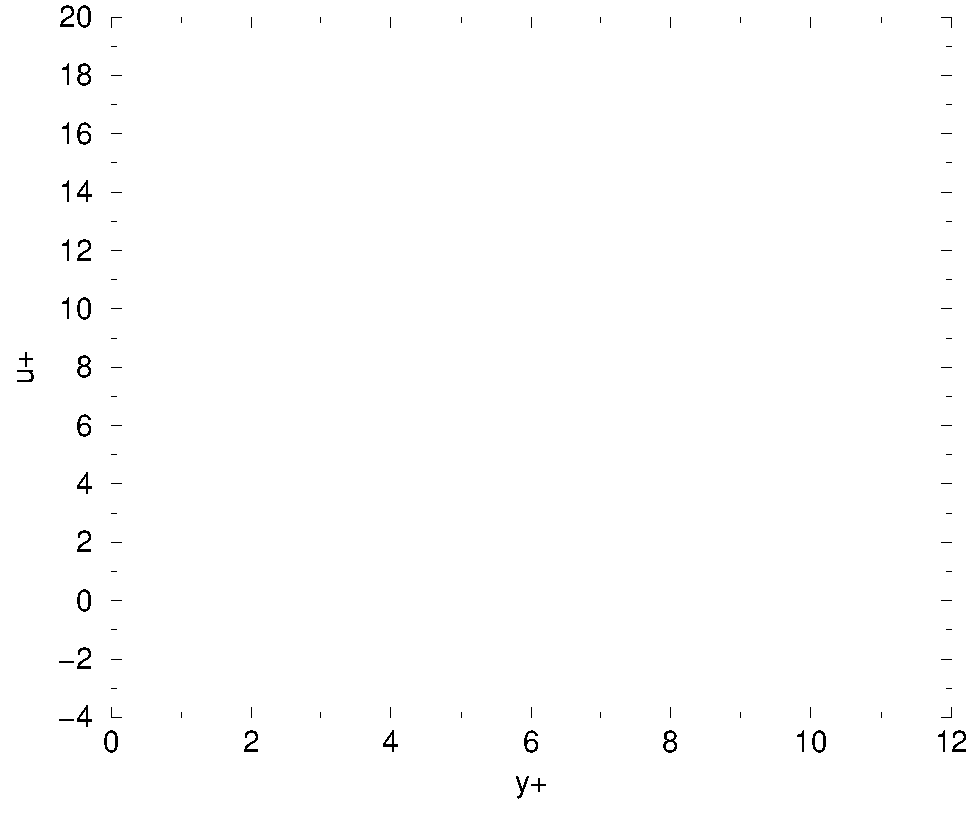
\includegraphics[height=7cm]{../Base/Clptur/Images/loilog.pdf}}
%\caption{\label{Base_Clptur_fig_loi_log_clptur}D\'etermination de $y^+$.}
%\end{figure}



% Plus d'actualite a priori, mais pistes de reflexion quand meme
%La limitation par valeur minimale de la vitesse dans (\ref{Base_Clptur_eq_ugrad_clptur}) 
%a \'et\'e corrig\'ee dans la version 1.1.0.q. 
%Auparavant, la formulation \'etait susceptible de conduire 
%\`a une valeur trop faible du gradient de vitesse et donc de la production
%turbulente en paroi. Elle s'\'ecrivait~: 
%\begin{equation}
%u_{\tau,F,grad} =u_{\tau,I'}-\displaystyle\frac{u^*}{\kappa}min\left[max\left(1,
%2\sqrt{\displaystyle\frac{\rho_I\kappa\, u_k I'F}{\mu_{t,I}}
%}-\displaystyle\frac{1}{2}\right),ln\frac{2}{\kappa}+5,2\kappa\right] 
%\end{equation} 
%La  formulation a \'et\'e modifi\'ee~: 
%\begin{equation}\notag
%u_{\tau,F,grad} =max\left(u^*(\frac{1}{\kappa}ln\displaystyle\frac{2}{\kappa}+5,2), 
%u_{\tau,I'}-\displaystyle\frac{u^*}{\kappa}\left[max\left(1,
%2\sqrt{\displaystyle\frac{\rho_I\kappa\, u_k I'F}{\mu_{t,I}}
%}-\displaystyle\frac{1}{2}\right)\right]\right) 
%\end{equation}
%Elle a \'et\'e adopt\'ee apr\`es des tests sur des
%configurations de validation (canal, marche descendante,  jet impactant, dune,
%echo, rra) qui n'ont montr\'e aucune influence de la modification. 
%\`A partir de la version 1.1.0.t, on a utilis\'e la valeur 
%$y^+_\text{lim}=10,88$ et non plus $\frac{2}{\kappa}$ pour caract\'eriser le
%passage de la loi lin\'eaire \`a la loi logarithmique et la 
%relation a donc \'et\'e modifi\'ee comme suit~: 
%\begin{equation}\notag
%u_{\tau,F,grad} =max\left(u^*(\frac{1}{\kappa}ln(y^+_\text{lim})+5,2), 
%u_{\tau,I'}-\displaystyle\frac{u^*}{\kappa}\left[max\left(1,
%2\sqrt{\displaystyle\frac{\rho_I\kappa\, u_k I'F}{\mu_{t,I}}
%}-\displaystyle\frac{1}{2}\right)\right]\right) 
%\end{equation}
%Comme, pour des $y^+$ inf\'erieurs \`a $y^+_\text{lim}$, on applique une 
%condition d'adh\'erence, cette approche n'est pas continue au voisinage de 
%$y^+_\text{lim}$. Il serait utile de se pencher sur la question. 
%Il faut cependant garder \`a l'esprit que la condition 
%de Dirichlet pour $k$ est prise nulle quand  $y^+$ est inf\'erieur \`a 
%$y^+_\text{lim}$, ce qui tend \'egalement \`a annuler la production, 
%quelle que soit la condition \`a la limite utilis\'ee pour la vitesse. 

Pour la loi thermique avec des nombres de Prandtl tr\`es petits devant 
l'unit\'e, Arpaci et Larsen sugg\`erent de prendre $y_0^+ \simeq 5/Pr$ 
(en s'appuyant sur des donn\'ees exp\'erimentales) plut\^ot que
$Pr_t/(Pr\,\kappa)$ (valeur adopt\'ee actuellement et 
issue de l'intersection analytique des lois 
lin\'eaire et logarithmique consid\'er\'ees). Il faudrait se pencher sur 
la question. 
